% sec_sound.tex
\section{Скорость звука в Свободном эфире}

\begin{figure}[h]
\centering
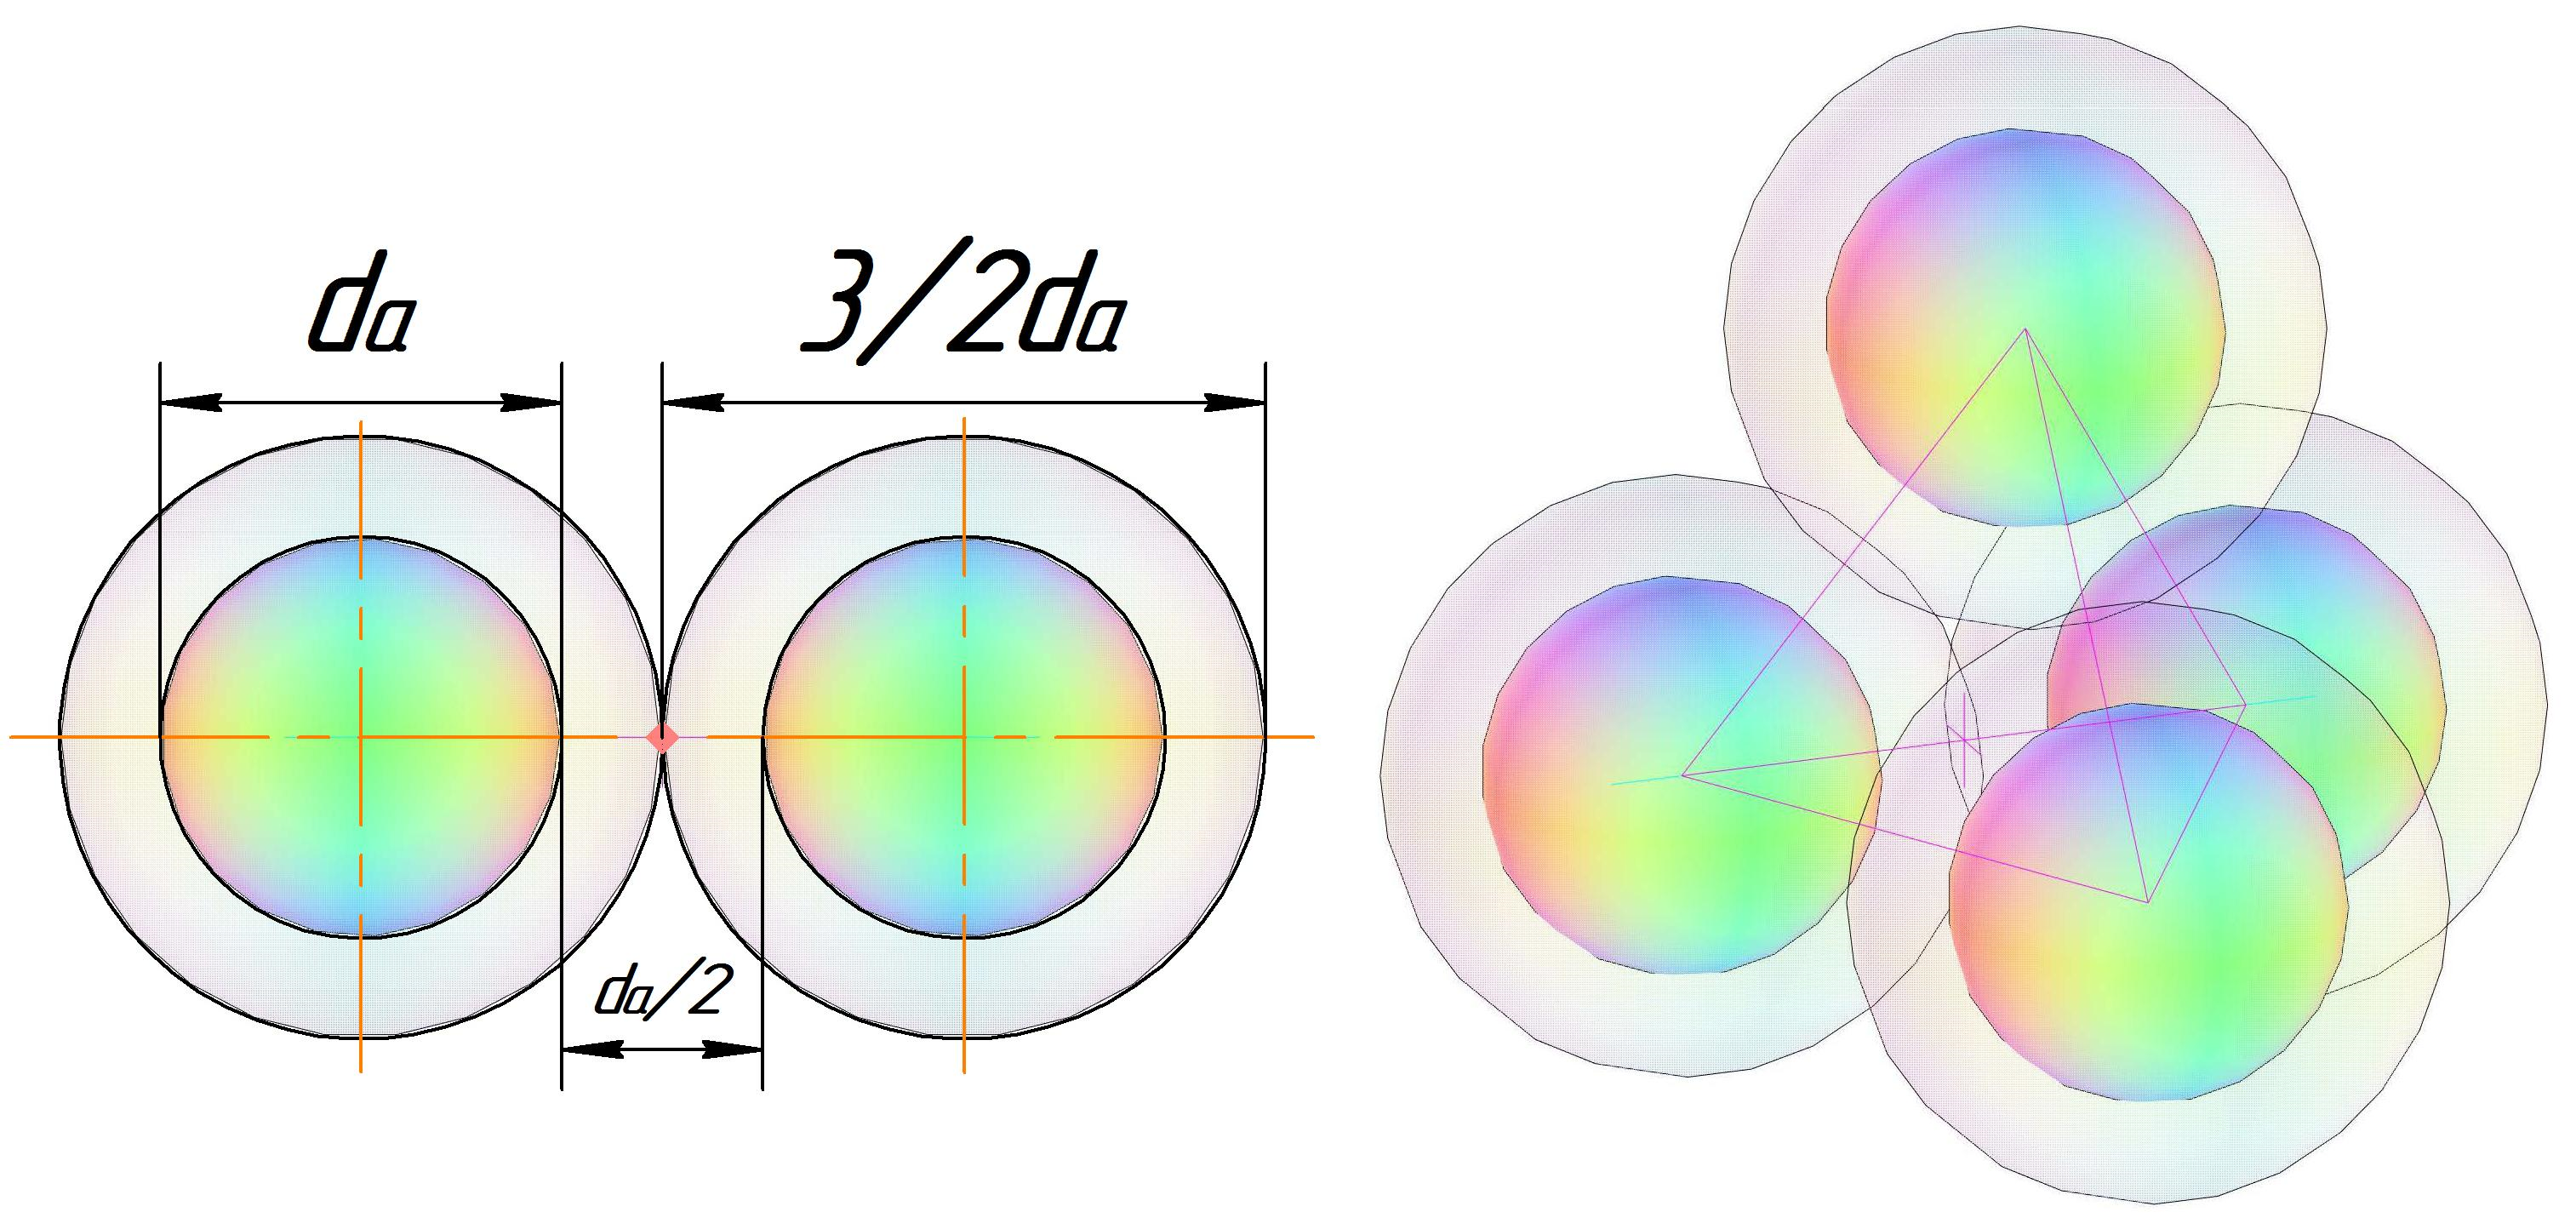
\includegraphics[width=0.5\textwidth]{images/a20.png}
\caption{Схема расчёта скорости звука в СЭ.}
%\label{fig:sliding_diagrams}
\end{figure}

Минимальный перенос (1,5\(d\)) реализуется, когда относительная скорость \(\mathbf{w}\) идёт почти по касательной — точка контакта «скользит» вдоль экватора полусфер. Максимальный (2,5\(d\)) — когда \(\mathbf{w}\) направлена вдоль линии центров; две крайние «активные» точки лежат на противоположных концах диаметра. Удобно считать, что длина «шага» линейно зависит от угла \(\theta\) между \(\mathbf{w}\) и радиус-вектором до точки контакта:
\[
L(\theta) = d_a + \frac{d_a}{2} \sin\theta = d_a\left(1 + \frac{\sin\theta}{2}\right).
\]

Угловое усреднение: для изотропного приближения плотность вероятности \(P(\theta) = 2\cos\theta\,\sin\theta\) (половина сферы). Среднее:
\[
\langle L \rangle = d_a \int_{0}^{\pi/2} \left(1 + \frac{\sin\theta}{2}\right) 2\cos\theta\sin\theta\,d\theta = d_a \left[ \frac{1}{2} + \frac{1}{3} \right] = \frac{5}{6}d_a.
\]

Время одного «шага»:
\[
\Delta t = \frac{\langle L \rangle}{\sqrt{2}\,v_0} = \frac{5d_a}{6\sqrt{2}\,v_0}.
\]

Скорость фронта возмущения:
\[
v_s = \frac{\langle L \rangle + d_a}{\Delta t} = \frac{\frac{5}{6}d_a + d_a}{\frac{5d_a}{6\sqrt{2}\,v_0}} = \frac{\frac{11}{6}d_a}{\frac{5d_a}{6\sqrt{2}\,v_0}} = \frac{11}{5}\sqrt{2}\,v_0 = 2.2\sqrt{2}\,v_0 \approx 3.111\,v_0.
\]

Что получилось: истинная скорость звукового фронта в Свободном эфире, учитывая блуждание точки столкновений, действительно лежит среднее между двумя крайними оценками и даётся удобной величиной
\[
v_s \approx 3,111\,v_0.
\]


